The metal films were fabricated using plasma sputtering.  The standard
process consisted of top-down sputtering in Argon plasma at a pressure of
\SI{1}{\milli\torr} and a flow rate of \SI{12}{STP}.  The deposition rates
were \SI{6.60}{\angstrom\per\second} for gold and
\SI{5.88}{\angstrom\per\second} for silver at 150 and \SI{66}{\watt} DC,
respectively.  During sputtering, the samples were rotated at \SI{50}{RPM}.
Though adhesion of the metal films to both glass and fluoropolymer
substrates was poor, instances of in-situ film-substrate separation were
rare (4-5 times amongst hundreds of experiments).  Film-substrate
separation was observed to be instigated by stresses caused by pressure
differentials in the microfluidic flow cell.  The majority of such stresses
were mitigated by employing the siphon effect to flow liquids in the
microfluidic cell in lieu of mechanically forced flow.

%\begin{figure}
%\centering
%\includegraphics[keepaspectratio,width=5cm]{experimental/figures/SEM-nanoparticles.pdf}
%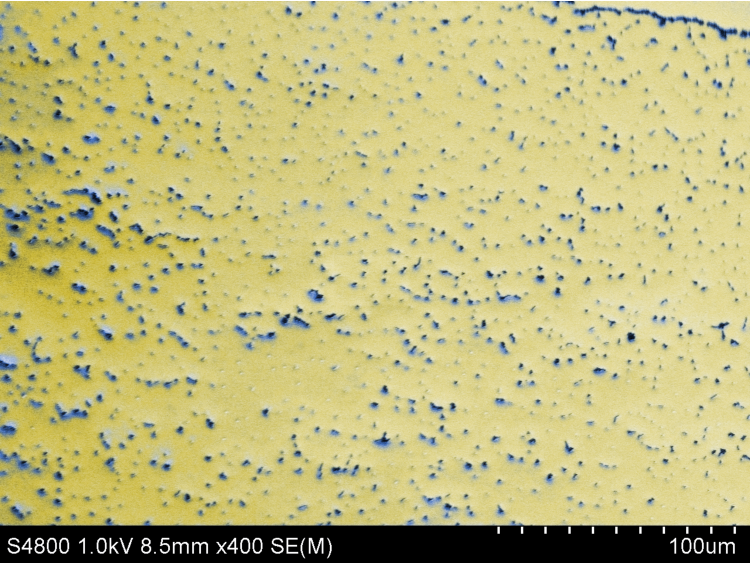
\includegraphics[keepaspectratio,width=5cm]{experimental/figures/SEM-holesa.pdf}
%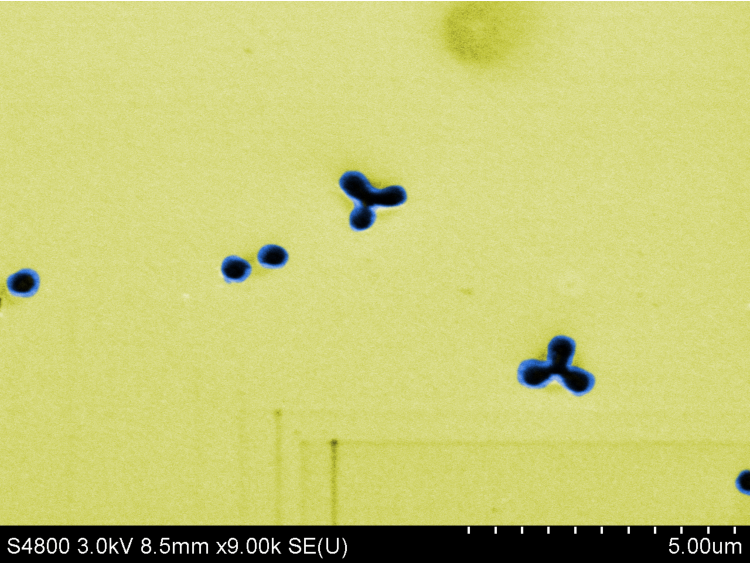
\includegraphics[keepaspectratio,width=5cm]{experimental/figures/SEM-holesb.pdf}
%\caption{SEM images of typical films produced with the plasma sputtering
%technique using the base set of parameters described in the text.}
%\label{fig:semsputter}
%\end{figure}

The substrate material consisted of a \SI{12}{\milli\meter} diameter BK7 No
1 glass coverslip.  Coverslips were cleaned in a hot base bath.  A
\SI{2}{\percent} solution of Hellmanex II was first prepared in a pyrex
beaker with a volume of \SI{25}{\milli\liter} and heated to a temperature
of \SI{60}{\celsius} on a hot plate.  The BK7 slides were immersed for
\SI{300}{\second}.  The beaker was then removed from the hot plate and put
in a sonicator for \SI{300}{\second}.  After sonication, the slides were
removed from the solution and washed liberally with distilled water and
dried under a dry nitrogen stream.  Cleaned slides were stored individually
on top of a small \SI{1}{\milli\meter\cubed} piece of PDMS plasma bonded to
a microscope slide. Batches of prepared slides were kept in a dark box
until use.  Slides sputtered with metal films were stored in the same
manner, but always used within one or two days to forestall contamination
or possible oxidation in the case of silver films.

\subsection{Prisms}
Hemispherical prisms of several different materials were employed over the
course of the experimental work.  The most common was glass, either LAH79
or BK7 upon which the metal was deposited directly.  Such glass prisms were
prepared by first removing any existing metal film.  Silver films were
removed by immersion in \SI{70}{\percent} \ce{HNO3} for \SI{60}{\second}.
Gold films were removed similarly by immersion in freshly prepared aqua
regia, composed of a 1:3 ratio of \ce{HNO3} to \ce{HCl}.  The glass prisms
were then sonicated in acetone to remove any organic contaminants and
rinsed in ultra-pure dry acetone.  Finally, the surface was cleaned with
methanol and lens tissue using the drag and drop method.

For reasons of experimental convenience, disposable hemispheres made of 
NOA89 optical UV adhesive were also employed.

.  To do this, BK7 glass
hemispheres were immersed in PDMS to create a mould.  Once the glass
hemisphere was removed, the void was filled with NOA89 and cured under a
\SI{15}{\watt} UV lamp at a distance of \SI{5}{\centi\meter} for
\SI{12}{\hour}.  To remove bubbles, the UV adhesive was first centrifuged
in an opaque microcentrifuge tube at \SI{15000}{RPM} for \SI{30}{\minute}.

In our experiments we found no observable difference between hemispheres
made of glass or ones cast with UV adhesive; we therefore do not
differentiate between the two in our discussion.  
